\section{(not actually a) Literature review}
\label{sec:gc:litreview}

There are two ways of thinking about graph comparison. Let $\hat{G^1}(V^1,E^1), 
\hat{G^2}(V^2,E^2)$ each be some labeled graph. 

\tablespacing
\begin{enumerate}
	\item \textbf{Graph summarization:} Compute some vector 
	$\overrightarrow{v^1}$ on $\hat{G^1}$ 1 that ``summarizes'' some property 
	it has. Similarly, compute $\overrightarrow{v^2}$ on $\hat{G^2}$ to capture 
	the same property that $\overrightarrow{v^1}$ does. Finally, compute 
	$f(\overrightarrow{v^1},\overrightarrow{v^2})$ where $f$ is some distance 
	function (e.g. Euclidean distance). A high value indicates strong 
	dissimilarity while a low value indicates similarity. 
	
	\item \textbf{Graph distance:} Create a valid distance function $f$ on the 
	graphs $\hat{G^1}, \hat{G^2}$ directly rather than a vector of metrics 
	($\overrightarrow{v^1},\overrightarrow{v^2}$). 
	Compute $f(\hat{G^1},\hat{G^2})$. Again, a high value indicates strong 
	dissimilarity while a low value indicates similarity. 
\end{enumerate}
\bodyspacing

We focus on the graph summarization comparison method because it fulfills both 
desired criteria for the visualization system. To be more specific, we seek to 
better understand existing graph summarization methods: the qualities that each 
metric reveals about a graph and associated advantages and drawbacks. 
Understanding these metrics is important due to the complex nature of graphs.
It is natural to ask why one cannot plot the graphs themselves (which are 
typically in the form of either an adjacency matrix of list of edges) and 
examine the result for visual patterns in order to understand the qualities 
of the graph. This is unfeasible for several reasons (see 
Figure~\ref{fig:gc:arr_density}). 

\tablespacing
\begin{itemize}
	\item \textbf{Arrangement:} Different arrangements of nodes on the visual 
	plane may have a profound effect on the interpretability of the graph; it 
	is unclear what the best arrangement might be at the start, and it is 
	unfeasible for an analyst to simply try all possible arrangements 
	especially as the number of variables increase.
	
	\item \textbf{Density:} The more nodes there are, the more edges there may 
	be, and the more dense a graph may become, making it incredibly difficult 
	to interpret. Furthermore, it makes it more difficult to find anomalies 
	among the variable's relationships (represented by edges). A non-existent 
	edge in a dense graph is just as important as an existent edge in a sparse 
	graph as each indicates a relationship which isn't quite like all the 
	others.
\end{itemize}
\bodyspacing

\begin{figure}[htb]
	\begin{center}
		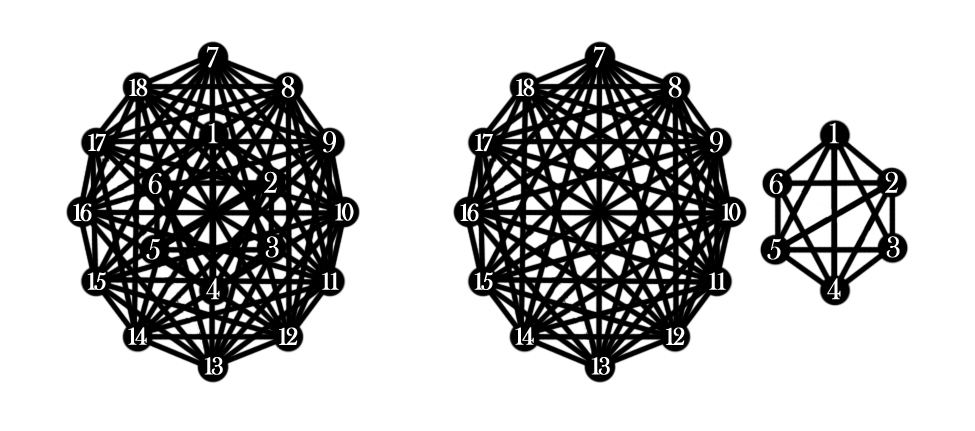
\includegraphics[width=1\linewidth]{ch-gc/figures/arr_density}
		\caption[Difficulties with graph visualization.]{
		Suppose we have a cluster graph $G(V = 18,E)$ with clusters $C^1,C^2$. 
		Let $C^1$ be composed of nodes $(V_1,...,V_6)$, and $C^2$ be composed 
		of nodes $(V_7,...,V_{18})$. 
		\textit{Left:} $C^1$, the smaller cluster, has been placed inside 
		$C^2$, the larger cluster. It is difficult to discern any meaningful 
		patterns; each node appears to be connected to every other node as the 
		density of the cluster $C^2$ makes it almost impossible to see that of 
		$C^1$.
		\textit{Right:} The nodes have been rearranged in a manner that clearly 
		distinguishes between $C^1$ and $C^2$. At a glance, it is evident that 
		$C^1$ is missing $E_{3,6}$. It is difficult to tell, however, that 
		$C^2$ is even missing an edge in the first place! It just so happens 
		that $E_{13,17}$ is the missing edge.
		$C^1$ is more sparse, which makes it easier to visually perceive 
		anomalies in the data.}
		\label{fig:gc:arr_density}
	\end{center}
\end{figure}

Graph summarization acts as a ``proxy'' for visually exploring the graph 
itself, and each metric can be ``parsed'' and combined afterwards to 
``reconstruct'' or better understand the qualities of each graph, subsequently 
allowing the user to better understand \textit{exactly where} the visual and 
numeric graphs differ (should the final graph comparison metric suggest that 
the two graphs are highly different). Graph distance functions skip that 
critical step which enable this level of analysis by going through the graphs 
directly.

To put it in another way, graph summarization has the \textit{exact opposite 
problem} that is present in data analytics as it is practiced today (discussed 
in Chapter~\ref{ch:intro}, this is the motivation behind the VS and this work). 
The VS allows the user to use visual qualities of a plot (many plots) to better 
understand numerical methods while graph summarization allows the user to 
numerical methods to better understand the visual qualities of a graph. 

With an understanding of the properties of various graph summarization methods, 
the graph summarization method results may be better interpreted. The method 
computes a list of metrics $(l^1,l^2)$ for each graph in order to provide a 
single vector $\overrightarrow{d^{1,2}}$ that quantifies the difference 
between the two graphs with some function (e.g. Euclidean distance, L2, etc.). 
As such, a natural byproduct of the computation is $(l^1,l^2)$, which (armed 
with an understanding of the values) provide insights on the qualities of the 
visual graph and numeric graph \textit{on an individual level} and where 
exactly their differences and similarities lie.